\documentclass[10pt,twocolumn,letterpaper]{article}

\usepackage{cvpr}
\usepackage{times}
\usepackage{epsfig}
\usepackage{graphicx}
\usepackage{amsmath}
\usepackage{amssymb}
\usepackage[utf8]{inputenc}
\usepackage{cite}
\usepackage{listings}
\usepackage[portuguese,ruled,lined]{algorithm2e}
\usepackage{spverbatim}
\usepackage{graphicx}
\usepackage{times}

\renewcommand{\figurename}{Fig.}
\renewcommand{\refname}{Referências}
%\renewcommand{\familydefault}{Computer Modern}
%\usepackage[breaklinks=true,bookmarks=false]{hyperref}

%\DeclareMathSizes{10}{20}{10}{10}

\cvprfinalcopy

\def\cvprPaperID{****}
%\def\httilde{\mbox{\tt\raisebox{-.5ex}{\symbol{126}}}}


\setcounter{page}{1}
\begin{document}

\title{\Huge Utilização do algoritmo PSO para ajuste dos pesos em redes RBF}

\author{Daniel Vilas-Boas\\
\footnotesize Departamento de Estatística e Informática\\
\footnotesize Universidade Federal Rural de Pernambuco\\
{\tt\small daanielvb@gmail.com}
\and
Leonardo Figueiroa\\
\footnotesize Departamento de Estatística e Informática\\
\footnotesize Universidade Federal Rural de Pernambuco\\
{\tt\small leonardofigueiroa@live.com}
\and
Rodrigo Cunha\\
\footnotesize Departamento de Estatística e Informática\\
\footnotesize Universidade Federal Rural de Pernambuco\\
{\tt\small r-cunha@outlook.com}
}

\maketitle
%\thispagestyle{empty}

\begin{abstract}
O uso de redes neurais de base radial ou RBFs vem sendo bastante utilizadas para classificação de padrões por apresentar diversas vantagens sobre outras redes (como a MLP), apresentando um treinamento mais eficiente e melhor grau de separabilidade. Este trabalho envolveu o desenvolvimento de uma RBF em conjunto com o algoritmo de otimização por enxame de partículas ou PSO. A rede neural foi desenvolvida de forma que seus pesos de saída fossem ajustados pelo PSO visando obter os melhores pesos na camada de saída e consequentemente menor taxa de erro e melhor classificação das características de entrada.\\
\begin{center}
\textbf{\textit{Palavras-chave --- RBF; PSO; redes neurais; classificação de padrões}}\\
\end{center}
\end{abstract}


\section{Introdução}
As redes denominadas \textit{funções de base radial}, convencionalmente conhecidas como \textit{RBF (radial basis function)}, são usadas em variados tipos de problemas tais como aproximação de funções e classificação de padrões. Ela pertence a arquitetura \textbf{feedforward} de camas múltiplas, cujo treinamento é efetivado de forma supervisionada. Sua estrutura é composta tipicamente por apenas uma camada intermediária, na qual as funções de ativação são do tipo \textit{gaussiana}. O fluxo de informações tem início na camada de entrada, passando então pela respectiva camada intermediária, e finalizando na camada neural de saída com neurônios com funções de ativação linear~\cite{livroAula}.\\ 

O \textit{PSO (Particle Swarm Optimization)} é um algoritmo de otimização por enxame de partículas. Tem uma abordagem \textbf{estocástica}, baseada em população que simula o processo comportamental de interação entre os indivíduos de um grupo. Sua teoria é baseada em comportamento de atividades de grupos de animais como pássaros e peixes, que realizam tarefas de otimização na execução de atividades como a busca por alimentos. O \textit{PSO} se inicia com um enxame de partículas com posições aleatórias. Cada partícula é dita ser uma possível solução para o problema investigado, sendo atribuído a cada indivíduo (partícula) um valor que está relacionado a adequação da partícula com a solução do problema (denominada \textbf{fitness}), e, também, uma variável velocidade que representa a direção do movimento da partícula. Com o passar do tempo, as partículas vão ajustando suas velocidades em relação a seu melhor \textbf{fitness}, encontrada pela própria partícula, e também pela melhor solução do grupo de partículas.\\ Elas continuam realizando este processo até que encontrem uma solução ótima. O valor \textbf{fitness} é definido pela natureza do problema de otimização e é computada por uma função objetivo que avalia um vetor solução. \\

Neste papel são discutidos a implementação da rede neural \textit{RBF} em conjunto com o algoritmo de otimização \textit{PSO}, os experimentos realizados após a implementação, e os resultados encontrados após os experimentos realizados.


%-------------------------------------------------------------------------
\subsection{Procedimentos}
Nesta seção serão discutidos os procedimentos realizados pela rede neural e pelo algoritmo de otimização. Os procedimentos são outros algoritmos conhecidos na literatura de \textbf{inteligência artificial} e \textbf{redes neurais artificiais} (como o \textit{kMeans} e a \textit{RBF}). Serão brevemente discutidos como funcionam e o seu papel na implementação do projeto. No \textbf{apêndice} pode ser encontrado o código-fonte do projeto para eventual consulta. O código-fonte está escrito em linguagem \textit{Java}.

\subsection{kMeans}

O primeiro procedimento realizado foi a \textbf{clusterização} das amostras por meio do algoritmo \textit{kMeans}. A partir de um valor $n$ que representa o número de centros na camada escondida da \textit{RBF} o algoritmo realiza a separação das amostras, calculando $n$ centros e suas respectivas variâncias.

\subsection{Radial Basis Function --- RBF}
Diferentemente das redes neurais do tipo \textit{MLP}, as redes do tipo \textit{RBF} possuem uma única camada escondida, cujos neurônios são constituídos de \textbf{funções de base radial}. O aprendizado neste tipo de rede é equivalente a encontrar uma superfície no espaço que forneça o melhor ajuste para os dados de treinamento. A estrutura típica de uma rede de função de base radial possui uma cama de entrada que está associada diretamente às informações de entrada da rede, uma única camada escondida constituída por funções de ativação de base radial que realizam uma transformação não-linear do espaço de entrada, e uma camada de saída linear que fornece a resposta ao padrão aplicado nas entradas da rede, conforme a figura abaixo.
\begin{figure}[h]
\begin{center}
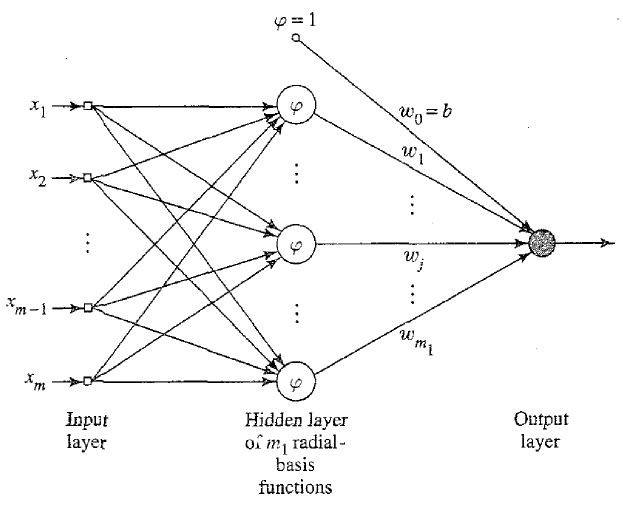
\includegraphics[scale=0.3]{foto1.jpg}
\caption{\textit{Estrutura teórica da RBF}}
\end{center}
\end{figure}
Nas redes neurais do tipo \textit{RBF} as informações das funções da camada escondida são determinadas pela distância, normalmente \textit{euclidiana}, entre o vetor de entrada e o centro daquela unidade. Ou seja, as variáveis de entrada constituem os dados utilizados pelas funções de ativação da rede, onde os pesos que conectam as camadas de entrada e escondida podem ser considerados unitários.
A camada de saída \textbf{não} contém funções de ativação, ela é considerada uma combinação linear que é dada pela soma ponderada dos valores gerados pelas funções de ativação das unidades escondidas, que são multiplicados pelos correspondentes pesos da camada de saída da rede.

\subsection{Cálculo das saídas intermediárias --- Y}

A partir dos centros das amostras e suas respectivas variâncias é utilizada a \textbf{função de base radial} para determinar o valor de saída da camada intermediária. A fórmula é dada abaixo:
\begin{equation}
\Large{e^{- \frac{(u - c)^2}{2\sigma^2}}}
\end{equation}

Onde \large{$e$} é a função exponencial de $(u-c)^2$ que é a \textbf{distância euclidiana} entre centro ($c$) e as amostra ($u$), pela \textbf{variância} ($\sigma$) ao quadrado multiplicada por 2.

\subsection{Particle Swarm Optimisation --- PSO}
A otimização através de enxame de partículas é uma técnica \textbf{estocástica} baseada em processos comportamentais de grupos de animais criada pelo \textit{Dr. Eberhart} e  \textit{Dr. Kennedy} em 1995. O \textit{PSO} possui várias similaridades com as técnicas evolucionárias como os \textbf{Algoritmos Genéticos}, pois utiliza o conceito de vida artificial para interpretar comportamentos biológicos. Porém, apesar de possuir algumas similaridades como inicialização aleatória da população, a presença de um fator comparativo para avaliar a população (fitness) e atualização da população à medida que procuram pela solução ótima, diferenciam-se quanto a presença de operadores evolucionários como o \textbf{crossover} e a \textbf{mutação}. Isso resulta na evolução apenas da procura pela solução ótima e nao dos organismos em si.\\
O conceito é gerar uma coleção de partículas dentro de um espaço de função cujas dimensões são variáveis com o número de neurônios da camada escondida da \textit{RBF}. Cada partícula, então, segue o líder do enxame através da melhor partícula global em cada iteração, atualizando sua velocidade (e consequentemente sua posição) através das equações $(a)$ e $(b)$ que serão discutidas em breve. Nessa implementação \textbf{não} foram consideradas topologias de vizinhança para as partículas.~\cite{xiao}\\Abaixo, segue o algoritmo em pseudo-código do procedimento.
\newpage
\begin{algorithm}[h!]
\Inicio{
\ParaCada {particula}{
inicialize a particula\;
}
\Repita{número de épocas ser atingido}{
\ParaCada{particula}{
calcule o valor do fitness\;
\Se {fitness for melhor $(\leq)$ que o fitness em pBest}{
guarde o valor como o novo pBest\;
}
}
Escolha a particula com melhor valor de fitness de todas as particulas como a gBest\;
\ParaCada {particula}{
calcule a velocidade de acordo com a equação (a)\;
atualize a posição de acordo com a equação (b)\;
}
}
}
\caption{Pseudo-código do PSO}
\end{algorithm}

Após as partículas serem inicializadas no espaço de função (intervalo de $-1 a 1$) é calculado o valor do \textbf{fitness} de cada partícula. O cálculo do valor é feito pela \textit{RBF} como o percentual de erro, discutido na seção acima.
Após o fitness ter sido calculado definimos o melhor global, que age como um fator de liderança para as demais partículas, e o melhor local da partícula (fator inércia). A partir deles, podemos calcular os vetores resultantes auxiliares e depois o vetor velocidade final que irá atualizar a posição da partícula no espaço. As equações de cálculo da velocidade e atualização da posição seguem:

\begin{center}
\textit{(a)}\qquad$\vec{v} = \vec{v} + c_1 \times rand() \times (\vec{pBest} - \vec{pos}) + c_2 \times rand() \times (\vec{gBest - \vec{pos}})$ 
\end{center}

Onde $\vec{v}$ é o vetor velocidade, $c_1$ e $c_2$ são fatores de aprendizado ($c_1 = c_2 = 2$), $rand()$ é uma função que irá gerar um valor aleatório no intervalo 0 --- 1, $\vec{pBest}$ e $\vec{gBest}$ são os vetores de posição do melhor local e global respectivamente, e $\vec{pos}$ é o vetor posição atual da partícula. 

\begin{center}
\textit{(b)}\qquad$\vec{pos} = \vec{pos_{ant}} + \vec{v}$ 
\end{center}
Onde $\vec{pos}$ é o vetor posição atual da partícula a ser atualizado, $\vec{pos_{ant}}$ é o vetor posição anterior a atualização, e $\vec{v}$ é o vetor velocidade calculado através da equação $(a)$.
%-------------------------------------------------------------------------

\section{Experimentos}

\subsection{Variando o número de neurônios, épocas e partículas}
Pellentesque mauris sem, blandit tempor scelerisque nec, dictum sed lorem. Proin in libero a elit bibendum volutpat vitae a ligula. Aliquam sagittis ligula quis auctor sollicitudin. Sed eget blandit elit, ac sagittis dolor. Vestibulum in eros a nibh venenatis fermentum sit amet nec nibh. Suspendisse hendrerit cursus eros, eu ornare nisi placerat id. Phasellus venenatis eget velit eu consectetur. Sed elementum magna a venenatis cursus. Vivamus gravida viverra neque, et laoreet ipsum. Mauris pellentesque libero quis tincidunt ullamcorper. Donec egestas faucibus blandit. Morbi bibendum nibh eget dignissim congue. Sed maximus quis dolor quis congue. In hac habitasse platea dictumst.

Nullam pulvinar nunc nec interdum sodales. Cras elit erat, gravida id tortor eu, molestie volutpat felis. Duis quis ipsum sapien. Etiam nec porttitor est. Vestibulum neque leo, sagittis id interdum vitae, congue a mi. Vestibulum interdum ipsum id viverra egestas. Suspendisse iaculis turpis nibh, a viverra dolor tempor eget. Donec volutpat, sapien a auctor venenatis, justo enim gravida nisi, vitae laoreet ipsum ligula sit amet mauris. Proin rhoncus auctor lectus, in dignissim elit.

\subsection{Observações}
Nullam pulvinar nunc nec interdum sodales. Cras elit erat, gravida id tortor eu, molestie volutpat felis. Duis quis ipsum sapien. Etiam nec porttitor est. Vestibulum neque leo, sagittis id interdum vitae, congue a mi. Vestibulum interdum ipsum id viverra egestas.

\section{Conclusão}

Nullam pulvinar nunc nec interdum sodales. Cras elit erat, gravida id tortor eu, molestie volutpat felis. Duis quis ipsum sapien. Etiam nec porttitor est. Vestibulum neque leo, sagittis id interdum vitae, congue a mi. Vestibulum interdum ipsum id viverra egestas. Suspendisse iaculis turpis nibh, a viverra dolor tempor eget. Donec volutpat, sapien a auctor venenatis, justo enim gravida nisi, vitae laoreet ipsum ligula sit amet mauris. Proin rhoncus auctor lectus, in dignissim elit.

{\small
\bibliographystyle{ieee}
\bibliography{rna}
}
\end{document}
